\documentclass{article}
\newtheorem{thm}{Theorem}
\setlength{\oddsidemargin}{0.25in}
\setlength{\textwidth}{6in}
\setlength{\topmargin}{-0.25in}
\setlength{\headheight}{0.3in}
\setlength{\headsep}{0.2in}
\setlength{\textheight}{9in}
\setlength{\footskip}{0.1in}
\usepackage{multirow}
\usepackage{fullpage}
\usepackage{graphicx}
\usepackage{amsthm}
\usepackage{amssymb}
\usepackage{url}
\usepackage{amsfonts}
\usepackage{algpseudocode}
\usepackage{listings}
\usepackage{mathtools}

\usepackage{listings}
\usepackage{color}
 
\definecolor{codegreen}{rgb}{0,0.6,0}
\definecolor{codegray}{rgb}{0.5,0.5,0.5}
\definecolor{codepurple}{rgb}{0.58,0,0.82}
\definecolor{backcolour}{rgb}{0.95,0.95,0.92}
 
\lstdefinestyle{mystyle}{
    backgroundcolor=\color{backcolour},   
    commentstyle=\color{codegreen},
    keywordstyle=\color{magenta},
    numberstyle=\tiny\color{codegray},
    stringstyle=\color{codepurple},
    basicstyle=\footnotesize,
    breakatwhitespace=false,         
    breaklines=true,                 
    captionpos=b,                    
    keepspaces=true,                 
    numbers=left,                    
    numbersep=5pt,                  
    showspaces=false,                
    showstringspaces=false,
    showtabs=false,                  
    tabsize=2
}
 
\lstset{style=mystyle}


\begin{document}\title{Project 4: HBase WordCount\\ Cloud Computing\\ Spring 2017}         % Enter your title between curly braces
\author{Professor Judy Qiu }        % Enter your name between curly braces
\date{}          % Enter your date or \today between curly braces
\maketitle
\makeatother     % `@' is restored as a "non-letter" character
\pagestyle{plain}
\section*{Goal}
 
Write an HBase WordCount program to count all unique terms' occurrences from the clueWeb09 dataset. Each row record of columnfamily "frequencies" is unique; the rowkey is the unique term stored in byte format, column name is "count" and value is the term frequency shown in all documents. Load the result to HBase WordCountTable. Figure~\ref{fig:wordcounttablescheme} shows the schema of WordCountTable. You will compare the results of your finished run to a correct version we will supply to you.

\begin{figure}[!htbp]
\centering
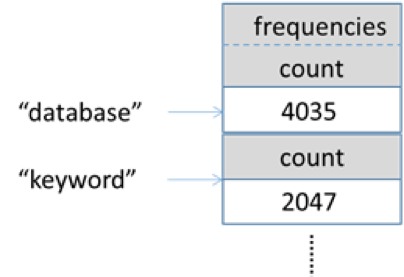
\includegraphics {wordcounttablescheme}
\caption{WordCount table schema for storing unique term's occurrences}
\label{fig:wordcounttablescheme}
\end{figure}


\section*{Deliverables}  
Zip your source code and report in a file named username\_project4.zip

\section*{Evaluation} 

The point total for this project is 1.5, where the distribution is as follows:
\begin{itemize} 
\item Correctness of your code and output (1 points)
\item	Completeness of written report (0.5 points)
\item	The report should explain the logic behind your code.
\end{itemize}
 

\section*{Prerequisites}
You?ll need to load data to HBase before trying this assignment. Please follow \textbf{project4\_Prereq.pdf} for more information. 


\section*{Introduction}

WordCount is a simple program which counts the number of occurrences of each word in a given text input dataset. It fits very well with the map/reduce programming model, making WordCount a great example to understand the Hadoop MapReduce programming style. Instead of loading the data from HDFS, we will load our data directly from existing HBase records which store the similar content structures on HBase and HDFS. 

In this homework and the next homework (Building an Inverted Index) we use the same source code, which can be found in: \textit{/root/MoocHomeworks/HBaseWordCount}.

\subsection*{Clueweb09 dataset}
We are using the ClueWeb09 dataset, which was created to support research on information retrieval and related human language technologies. It consists of about 1 billion webpages in ten languages that were collected in January and February 2009. The dataset is used by several tracks of the TREC conference\cite{Clueweb09}. Since the ClueWeb09 dataset is composed of webpages crawled from the Internet, the uploaded table schemas are designed as shown in Figure 2.

\begin{figure}[!htbp]
\centering
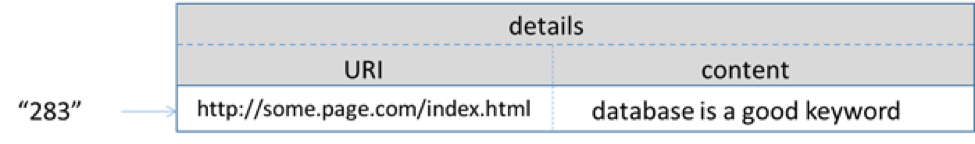
\includegraphics {datatablescheme}
\caption{Data table schema for storing the ClueWeb09 dataset}
\label{fig:datatablescheme}
\end{figure}

So, while similar to Hadoop WordCount \cite{hadoopwordcount}, the differences are that data is stored on HBase and URI is the "filename" that contains all the text content.


\subsection*{Mapper, Reducer and Main Program }

Now we are going to implement the HBase WordCount. Our implementation consists of three main parts:
\begin{itemize}
\item Mapper
\item Reducer
\item Main program
 \end{itemize}
 
 
\subsubsection*{Mapper}
A Mapper overrides the map function from the Class "org.apache.hadoop.hbase.mapreduce.TableMapper$<$Text, LongWritable$>$" which provides $<$key, value$>$ pairs as the input. A Mapper implementation may output $<$key, value$>$ pairs using the provided Context.
$<$key, value$>$ of this map function is $<$rowkey, content$>$, where the key is the rowkey of an HBase record related to a specified URI, and the content is the stored text of that URI. Your Map task should output $<$word, frequency$>$ for each word in the content of text.

\textit{Pseudocode}
\begin{lstlisting}[language=java] 
void Map (key, value){
    for each word x in the content of a hbase record:
    context.write(x, freq);
}
\end{lstlisting}
 
\textit{Detailed implementation}
\begin{lstlisting}[language=java] 
static class WcMapper extends TableMapper<Text, LongWritable> {
		@Override
		public void map(ImmutableBytesWritable row, Result result, Context context) throws IOException, InterruptedException {
			byte[] contentBytes = result.getValue(Constants.CF_DETAILS_BYTES, Constants.QUAL_CONTENT_BYTES);
			String content = Bytes.toString(contentBytes);
			
			// TODO: write your implementation for counting words in each row, and generating a <word, count> pair
			// Hint: use the "getWordFreq" function to count the frequencies of words in content
�
		}
}
\end{lstlisting}

\subsubsection*{Reducer}
A Reducer collects the intermediate $<$key, value$>$ output from multiple map tasks and assembles a single result. Here, the reducer function will sum up the occurrence of each word to pairs as $<$word, occurrenc$e>$, then write it back to an HBase table with put operations which contain the key-value pair information of each word.
\textit{Pseudocode}
\begin{lstlisting}[language=java] 
void Reduce (keyword, <list of value>){
    for each x in <list of value>:
        sum+=x;
        context.write(rowkey(x), freq);
}
\end{lstlisting}

\textit{Detailed implementation}
\begin{lstlisting}[language=java] 
public static class WcReducer extends TableReducer<Text, LongWritable, ImmutableBytesWritable> {
    	@Override
    public void reduce(Text word, Iterable<LongWritable> freqs, Context context)
                throws IOException, InterruptedException {
        /*TODO: write your implementation for getting the final count of each word
        and putting it into the word count table 
        Hint -- the schema of the WordCountTable is: 
           rowkey: a word, column family: "frequencies", 
           column name: "count", cell value: count of the word
        Check iu.pti.hbaseapp.Constants for the constant values to use.
	*/
    	long totalFreq = 0;
     }
}
 \end{lstlisting}
\subsubsection*{Main program }
The main function has been provided as standard initialization, although you can modify it to suit your own style. Hint: the provided code is designed for using put operations in the reducer content.write() function. Before writing the codes, please read the HBase MapReduce tutorial first \cite{hbaseexample}.



%\lstinputlisting[language=Java]{RunnerMap.java}

\section*{Edit}
 The sketch code is stored within the provided VirtualBox image Environment Setup. You may use linux text editor vi/vim to add your code.
 \begin{lstlisting}[language=bash] 
$ cd /root/MoocHomeworks/HBaseWordCount/
$ vim src/iu/pti/hbaseapp/clueweb09/WordCountClueWeb09.java
 \end{lstlisting}
 
\subsection*{Compile and run your code}
For your convenience, we have provided a one-click script compileAndExecWordCount.sh for compiling and execution. Standard error messages such as "compile errors, execution errors, etc." will be redirected on the screen. You may debug it based on the returned messages.
\begin{lstlisting}[language=bash] 
$ cd /root/MoocHomeworks/HBaseWordCount
$ ./compileAndExecWordCount.sh
\end{lstlisting}
 
\section*{View the result}  
The result is generated as /root/MoocHomeworks/HBaseWordCount/output/project1.txt. 
\begin{lstlisting}[language=bash] 
$ cd /root/MoocHomeworks/HBaseWordCount
$ cat output/project1.txt
\end{lstlisting}
\bibliographystyle{unsrt} 
\bibliography{project4}
\end{document}
